\documentclass[../main.tex]{subfiles}
\begin{document}
\chapter{Stato dell'arte}

In questo capitolo verranno discussi i principali lavori che sono stati fatti durante l'ultimo decennio in letteratura. Si procede col fornire un'introduzione preliminare sui concetti che verranno utilizzati durante questa tesi.

\section{Malware}
Il termine malware è una combinazione delle parole \textit{malicious} e \textit{software}. Il malware rappresenta quei programmi software progettati per danneggiare o effettuare azioni indesiderate su un sistema informatico. \cite{MalwareDef}

Gli obiettivi che può avere un malware sono molteplici e sono in continua evoluzione. Il malware, a seconda dello scopo per cui è stato creato e alle sue caratteristiche, viene classificato nei seguenti modi:

\begin{verse}
				\textbf{Virus} Prendono il nome dai virus in campo biologico e si comportano in modo analogo, sono programmi che si replicano sul computer che hanno infettato e si predispongono ad infettare nuovi computer mediante mezzi di trasmissione quali email e chiavette USB. \cite{VirusDef}
\end{verse}

\begin{verse}
				\textbf{Spyware} Il termine Spyware è una combinazione delle parole \textit{Spy} e \textit{Software}. È un software che viene installato sul computer della vittima a sua insaputa e che raccoglie informazioni. 
				Uno spyware è oggetto di controversia perchè può essere utilizzato negli ambienti lavorativi per controllare le ricerche dei dipendenti o per controllare l'attività dei propri figli su internet. Anche se utilizzato per scopi più innocui può comunque violare la privacy dell'utente. \cite{Spyware2} \newline
				Usi più scorretti di programmi spyware prevedono di tracciare la cronologia internet di un utente per inviare pubblicità mirata, accedere alle password degli account in uso sul computer infetto e/o alle informazioni bancarie. Le informazioni raccolte attraverso l'uso di spyware possono essere utilizzate in vari modi, l'uso più frequente e più remunerativo ad oggi è quello di rivendere tali informazioni a dei terzi. \cite{Spyware1}
\end{verse}

\begin{verse}
				\textbf{Backdoor} Tradotto letteralmente come \textit{porta sul retro}, è un metodo utilizzato per avere un accesso privilegiato e spesso segreto che aggira il sistema di autenticazione previsto. Lo scopo di una backdoor è quello di permettere una connessione in remoto al computer vittima per prenderne il controllo.				
\end{verse}

\begin{verse}
				\textbf{Trojan} Il cavallo di Troia fu una macchina da guerra che, secondo la leggenda, fu usata dai greci per espugnare la citta di Troia. Questo termine è entrato nel linguaggio comune per indicare uno stratagemma con cui penetrare le difese. Nell'ambito dei malware il trojan è un software che si nasconde all'interno di un altro programma all'apparenza innocuo e che, se eseguito, esegue anche il codice del trojan \cite{TrojanDef}.
				Oggi col termine trojan ci si riferisce principalmente ai malware ad accesso remoto. Spesso vengono utilizzati per installare backdoor sui sistemi bersaglio. \cite{TrojanPurpose}
\end{verse}

I malware erano inizialmente usati per compiere azioni dolose sia da hacker malintenzionati che dai governi per sottrarre informazioni personali, inviare spam e commettere frodi. \cite{ScopoMalware} \cite{MalwareRevolution}

L'evoluzione e lo sviluppo di internet hanno portato ad un incremento degli utenti connessi sempre maggiore. Questa crescita di internet ha spostato l'obiettivo dei malware che vengono usati sempre di meno per compiere azioni dolose. Fin dal 2003 la maggior parte dei malware sono stati creati per prendere il controllo dei computer dell'utente vittima per scopi illeciti \cite{MalwareRevolution}. Vengono usati computer zombie per l'invio di email di spam o per effettuare attacchi distribuiti Denial of Service (DDoS).


\section{Botnet}
Nella sua forma più semplice una Botnet è un gruppo di computer che sono stati infettati da un malware che consente al suo controller, detto anche master, di avere il controllo sulle macchine infettate. Le Botnet sono usate dal master per compiere operazioni illecite ad insaputa della vittima. Una volta infetto, il computer della vittima prende il nome di zombie. \cite{Botnet} \newline
Per aggiungere un computer ad una botnet si infetta il computer vittima con un malware che installa una backdoor in grado di consentire al master di avere accesso remoto al computer infettato dal malware.
Il master ha così accesso ad un sistema gigantesco di computer zombie pronti ad essere attivati ed eseguire i suoi ordini. Le botnet rilevate e studiate nella storia dimostrano come questi sistemi possano arrivare a contenere anche milioni di computer infetti. \cite{Botnet}

I componenti di una botnet sono i seguenti:

\begin{verse}
				\textbf{Master} Il master è il computer che ha creato la botnet e che ne ha il controllo remoto. È detto C\&C (Command and Control) il programma che dà i comandi da eseguire tramite un canale nascosto sul computer della vittima.
\end{verse}

\begin{verse}
				\textbf{Control protocol} Il protocollo utilizzato dal master per comunicare con i computer zombie.
\end{verse}

\begin{verse}
				\textbf{Computer zombie} Computer connesso ad internet che è stato infettato attraverso dei virus o trojan e che può essere utilizzato in modo remoto. 
\end{verse}

Nella figura seguente viene rappresentato una possibile architettura di una botnet. Il master è il computer che controlla in modo remoto i computer zombie attraverso dei server C\&C.
\begin{figure}[H]
				\centering
				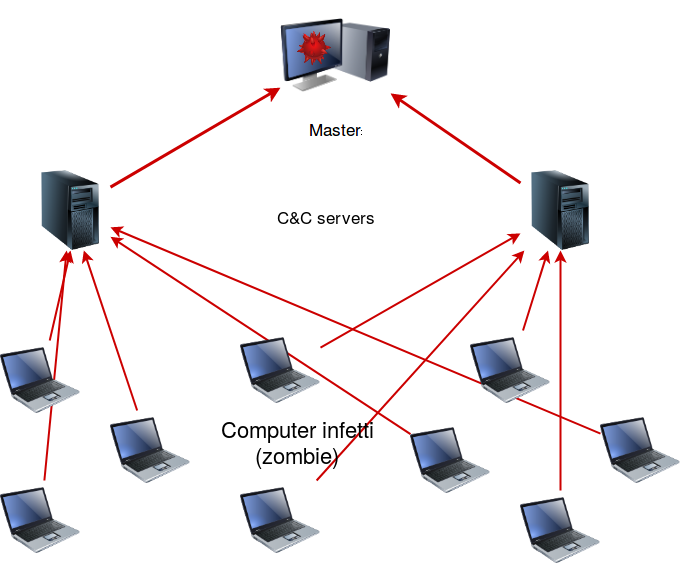
\includegraphics[scale=0.5]{botnet.png}
				\caption{Esempio architettura botnet}
\end{figure}

I principali attacchi informatici effettuati attraverso l'utilizzo delle botnet sono vari: possono essere spam, DDoS, click fraud e bitcoin mining per citarne alcuni. È quindi evidente come l'utilizzo delle botnet sia al fine di un guadagno economico.

\begin{verse}
				\textbf{Spam} È l'invio tramite posta elettronica di messaggi ad alta frequenza contenenti truffe o pubblicità.
\end{verse}

\begin{verse}
				\textbf{DDoS} Acronimo di Distributed Denial of Service, è un tipo di attacco in cui si mira a far esaurire le risorse di un sistema informatico affinchè non riesca più a fornire servizio. Per fare ciò si effettuano moltissime richieste al sistema per farlo rallentare o nei casi più estremi rendere inutilizzabile.
\end{verse}

\begin{verse}
				\textbf{Click fraud} Questo tipo di frode si verifica sulla pubblicità su internet di tipo pay per click. Questo tipo di pubblicità genera quantità di denaro in base al numero di click effettuati sull'annuncio pubblicitario. Le botnet sfruttano questo tipo di pubblicità utilizzando computer zombie per cliccare in massa gli annunci pubblicitari.
\end{verse}

\begin{verse}
				\textbf{Bitcoin mining} I bitcoin sono una criptovaluta che a differenza dei soldi, che vengono stampati da un governo centrale, vengono creati risolvendo operazioni matematiche complesse. Una botnet utilizza i computer zombie come unità di calcolo a cui far eseguire queste operazioni complesse.
\end{verse}

\section{Intrusion Detection System}
I sistemi di rilevamento delle intrusioni sono gli "allarmi antifurto" del campo della sicurezza informatica. L'obiettivo è difendere un sistema con un allarme che viene emesso ogni volta che la sicurezza del sito è stata compromessa. \cite{IDS} \newline

Un IDS è un dispositivo software o hardware utilizzato per identificare intrusioni a computer o reti locali.
Ci sono varie classi di intrusione che vanno rilevate: si possono verificare situazioni in cui un utente ruba una password, utenti legittimi che abusano dei loro privilegi o hacker che usano script trovati in rete per attaccare il sistema. Le intrusioni sono varie e non è possibile elencarle tutte.

Un IDS è composto da quattro componenti \cite{idsbook}:

\begin{itemize}
				\item \textbf{Sensori}, sono utilizzati per ricevere informazioni dalla rete o dai computer.

				\item \textbf{Console}, utilizzata per monitorare lo stato della rete e dei computer.

				\item \textbf{Motore}, analizza i dati prelevati dai sensori e provvede a individuare eventuali falle nella sicurezza.

				\item \textbf{Database}, memorizza le regole utilizzate per identificare violazioni di sicurezza.
\end{itemize}

Di seguito è presente un'immagine che descrive i componenti di un IDS. I pacchetti in entrata e uscita dalla rete sono ricevuti da un sensore che raccoglie il traffico dati, successivamente il motore analizza i dati prelevati dai sensori con le regole presenti nel database.

\begin{figure}[H]
				\centering
				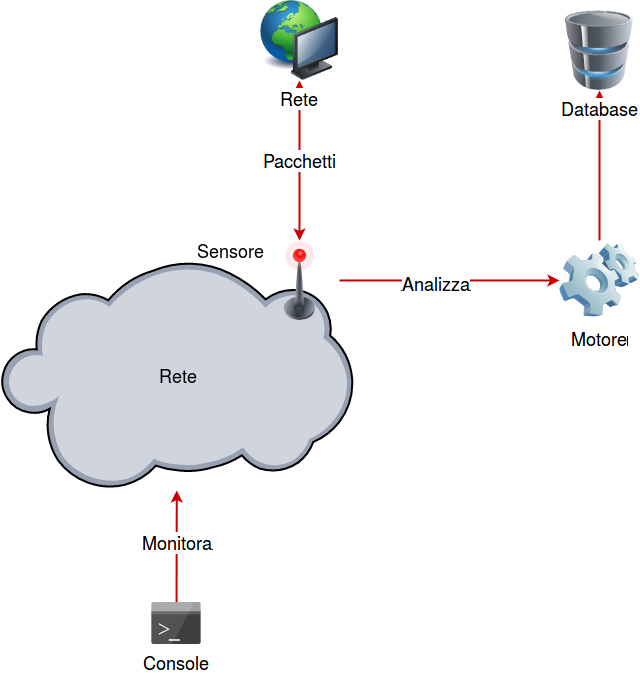
\includegraphics[scale=0.5]{IDS.png}
				\caption{Esempio di un IDS}
\end{figure}

Un IDS puó essere classificato in base al contesto a cui è applicato:

\begin{verse}
				\textbf{Network Intrusion Detection System (NIDS)} Il software è installato in punti che si interfacciano tra l'ambiente esterno e il segmento di rete da proteggere. In questo modo si fornisce una protezione su tutti i dispositivi presenti all'interno della stessa rete.
\end{verse}

\begin{verse}
				\textbf{Host Intrusion Detection System (HIDS)} Il software è installato su host singoli e monitora il traffico in entrata e uscita, se rileva un'attività sospetta avvisa l'utente.
\end{verse}

Le regole utilizzate per identificare le violazioni possono essere \cite{IDS}:

\begin{verse}
				\textbf{Signature detection} La decisione di rilevamento delle intrusioni è formata sulla base di un modello del processo intrusivo e di quali tracce dovrebbe lasciare nel sistema osservato. Questo metodo si basa sul presupposto che in qualsiasi caso riusciamo a definire un comportamento legale o illegale e confrontare di conseguenza il comportamento osservato.

				Un vantaggio di questo approccio è che avendo un modello con cui confrontare il comportamento che si sta osservando non esistono falsi positivi, ovvero quando si considera dannoso un comportamento innocuo generando un falso allarme, questo perchè i modelli comportamentali all'interno del database sono comportamenti per certo dannosi. È inoltre veloce e semplice in quanto si tratta soltanto di effettuare confronti con modelli illegali già noti.

				Uno svantaggio di questo approccio è che si possono verificare molti falsi negativi, cioè i comportamenti dannosi che non vengono segnalati. Questo si verifica perchè questi sistemi sfruttano regole per rilevare le intrusioni salvate su di un database, è quindi estremamente importante tenere aggiornato il database con tutti i possibili comportamenti dannosi.
\end{verse}

\begin{verse}
				\textbf{Anomaly detection} In questo tipo di rilevamento si parte con il presupposto che qualcosa di anormale sia molto probabilmente sospetto, si cercano quindi anomalie nel traffico. È quindi necessario uno studio anticipato della rete per capire cosa sia normale per il soggetto osservato. Si decide poi quanto è possibile discostarsi dal tipo di attività normale. Questo tipo di rilevamento guarda comportamenti che sono improbabili che si verifichino dallo studio effettuato sul traffico normale.  

				Il vantaggio di questo metodo è che indipendente dal tipo di intrusione ed è possibile utilizzare algoritmi di \textit{self learning} che apprendono da soli cosa è normale osservando il traffico per un lungo periodo di tempo.
\end{verse}



Esistono diversi tipi di tecniche per rilevare le intrusioni. In questa tesi si è fatto uso di un \textit{IDS} che utilizza algoritmi di \textit{machine learning}.

\textit{Machine learning} può essere definito come la capacità di un programma per computer di apprendere e migliorare le prestazioni su una serie di attività nel tempo. Le tecniche di \textit{machine learning} si concentrano sulla costruzione di un modello, \textit{behavioral model}, di sistema che migliora le sue prestazioni in base ai risultati precedenti. \newline


L'utilizzo di \textit{IDS} è un approccio utile per fare \textit{botnet detection} sul traffico di rete, si osserva il traffico di dati nella rete e si cercano comunicazioni sospette che possono essere fornite da \textit{bot}. \newline

\end{document}
